\section{Desenvolvimento de jogos}

Antes de se falar como se dá o desenvolvimento de jogos eletrônicos, é necessário definir o que é um jogo, quais os componentes que fazem parte de um jogo e como um jogo é estruturado.

Segundo Raph Koster \cite{koster2014a}, um jogo pode ser definido como uma experiência interativa que dá ao jogador uma série de padrões com desafios cada vez mais difíceis ao ponto que ele eventualmente os domine. Jogos diferentes contém temáticas diferentes, mecânicas diferentes e são executados em plataformas diferentes. Porém, a construção desses diferentes jogos tendem a ser bastante semelhante. Levando em consideração a semelhança de construção de jogos eletrônicos, Dave Roderick diz que “Um jogo é somente um banco de dados em tempo real com um front-end bonito” \cite[p.~625]{rollings2004game}.

Na próxima seção serão detalhados os componentes principais que compõem jogos eletrônicos.

\subsection{Componentes de um jogo}

De forma geral, um jogo é composto pelos seguintes módulos: vídeo, áudio, física, entrada, gerenciamento de recursos e eventos.

\begin{itemize}
\item \textbf{Módulo de vídeo:} módulo responsável por realizar a renderização de imagens, animações e textos. O vídeo de um jogo é composto por toda a parte de gameplay (onde o usuário está efetivamente jogando o jogo) e a parte de front-end, que, segundo Jason Gregory \cite[p.~39]{gregory2014game}, é composta pelo heads-up display (HUD), menus e qualquer interface de usuário presente no jogo.

\item \textbf{Módulo de áudio:} módulo responsável por realizar o gerenciamento de áudio no jogo. O áudio de um jogo é composto por músicas de fundo e efeitos sonoros.

\item \textbf{Módulo de física:} módulo responsável por simular a física do mundo real dentro do ambiente do jogo. A principal responsabilidade de um módulo de física é realizar a detecção de colisões entre objetos do jogo (personagens, cenários, chão, etc.)

\item \textbf{Módulo de entrada:} módulo responsável por coletar inputs advindos do jogador por meio de teclado, mouse, controles, etc.. Também chamado de módulo HID (human interface device), este pode ser simples ao ponto de somente coletar o pressionamento de botões, ou mais complexo, chegando a “detectar pressionamento de vários botões, sequências de botões pressionados e gestos, utilizando acelerômetros, por exemplo” \cite[p.~43]{gregory2014game}

\item \textbf{Módulo de gerenciamento de recursos:} Segundo Gregory \cite[p.~35]{gregory2014game}, este módulo é responsável por prover uma interface (ou conjunto de interfaces) unificada para acessar todo e qualquer tipo de recurso do jogo. Recurso do jogo, nesse caso, é qualquer imagem, script, fonte, áudio, mapa localizado nos arquivos do jogo, dentre outros.

\item \textbf{Módulo de rede:} não necessariamente utilizado em todos os jogos, porém importante ao ponto de ser citado, este módulo é responsável por prover suporte à comunicação (local ou online) entre diversos jogadores em um mesmo jogo.
\end{itemize}


Além dos componentes gerais, todo jogo contém um mecanismo que é responsável pelo controle do estado atual do jogo, conhecido como \textit{game loop}. Luciano Santos e Carla Castanho \cite{gameplayunb} caracterizam a estrutura de um game loop por quatro tipos de tarefas (utilizando como exemplo uma partida do jogo Tetris):

\begin{enumerate}
\item tarefas que serão executadas somente uma vez quando a partida iniciar como, por exemplo, zerar a quantidade de pontos e escolher uma peça inicial;
\item tarefas que serão executadas repetidamente (enquanto a partida não acabar) como, por exemplo, coletar inputs do jogador, verificar se o jogador completou uma linha no jogo, verificar se o jogador atingiu o topo da tela e atualizar a posição da peça que está caindo;
\item tarefas que serão executadas quando situações ou eventos específicos ocorrerem como, por exemplo, atualizar os pontos quando uma linha é completada;
\item tarefas que serão executadas somente uma vez quando o jogo estiver pronto para ser finalizado.
\end{enumerate}

\subsection{Arquitetura de um jogo}

Segundo Gregory, a separação entre um jogo e sua engine é uma linha turva \cite{gregory2014game}. Isso se dá principalmente pelo modo como é modelada a arquitetura do jogo. Caso seja utilizada uma arquitetura monolítica, a engine e o jogo serão um só, isto é, não haverá separação clara entre componentes genéricos e específicos do jogo. Por outro lado, caso o jogo utilize uma arquitetura sólida, esta separação é evidente.

\subsubsection{Arquitetura monolítica}

A primeira abordagem trata da construção do jogo utilizando um design de arquitetura monolítico. Nesta arquitetura cada objeto do jogo contém toda a sua implementação de mecânicas de renderização de gráficos, detecção de colisões, física, inteligência artificial, etc. Este modelo não é adequado para jogos mais complexos, pois, de acordo com Jeff Plummer \cite{jeffthesis}, o código não é reutilizável porque as mecânicas estão altamente acopladas com o comportamento dos objetos e, além disso, o design não é flexível, prejudicando a manutenção do código, pois qualquer modificação pode afetar o sistema inteiro.

\begin{figure}[H]
 \centering 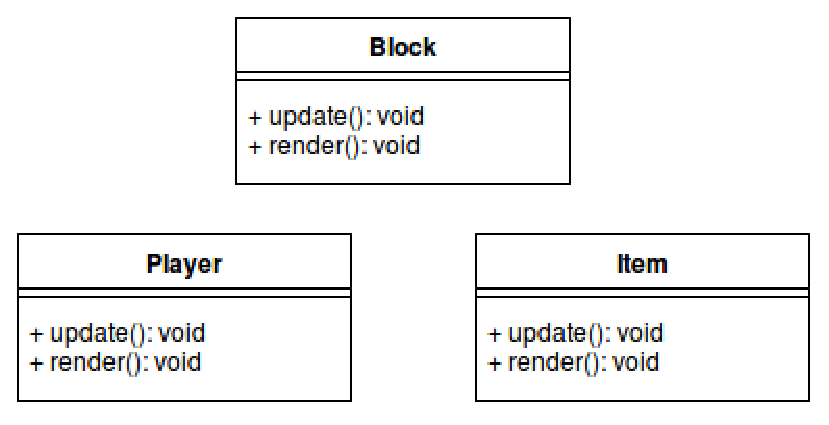
\includegraphics[keepaspectratio=true,scale=0.6]{figuras/monolithic-architecture.eps}
   \caption{Exemplo de arquitetura monolítica}
   \makebox[\width]{Fonte: \textit{Autores}.}
   \label{arch-monolitica}
\end{figure}

\subsubsection{Arquitetura reutilizável}

Esta arquitetura tem como objetivo principal desacoplar mecânicas gerais (como as já citadas acima) de objetos e funcionalidades específicas do jogo.

Segundo Rollings e Morris \cite{rollings2004game}, uma arquitetura bem implementada facilita a flexibilidade e reutilização de código, e mecânicas que tendem a mudar bastante durante o desenvolvimento do jogo estão atrás de uma interface consistente.

Rollings e Morris \cite{rollings2004game} definem esse modelo como “Arquitetura sólida” (do inglês, \textit{Hard Architecture}). Uma arquitetura sólida pode ser definida como um framework relativamente genérico que não necessariamente depende do tipo de jogo que é produzido utilizando-o, e é conciso e confiável em relação a suas interfaces, trazendo robustez à sua implementação.

\begin{figure}[H]
 \centering 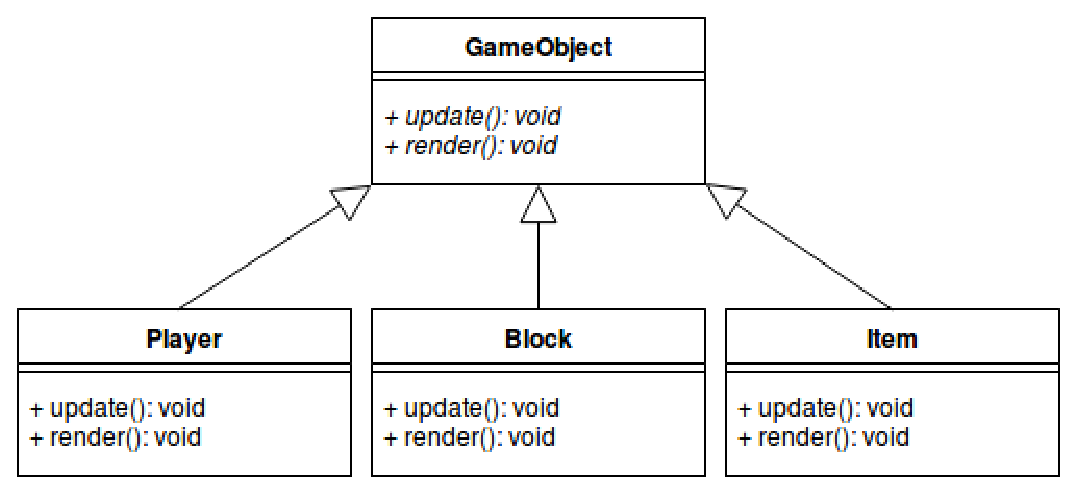
\includegraphics[keepaspectratio=true,scale=0.6]{figuras/reusable-architecture.eps}
   \caption{Exemplo de arquitetura reutilizável}
   \makebox[\width]{Fonte: \textit{Autores}.}
   \label{arch-reutilizavel}
\end{figure}

No modelo de arquitetura sólido, as mecânicas gerais do jogo estão definidas à parte e são providas interfaces para a utilização destas mecânicas. A partir dessa interface, as funcionalidades específicas do jogo são construídas. Esse conjunto de funcionalidades específicas do jogo é chamado de “Arquitetura Flexível” (do inglês, \textit{Soft Architecture}). Rollings e Morris \cite{rollings2004game} definem arquitetura flexível como “Uma arquitetura de um domínio específico, geralmente não reutilizada entre projetos diferentes, construída em cima da arquitetura sólida e fazendo o uso de seus serviços providos”.
